\section{Marco Teórico}

\subsection{Clasificación de los Instrumentos de Medición}

El contenido del presente marco teórico está basado en el recurso del Profesor Blondell~\cite{blondell}.

Existen diversos instrumentos para medir magnitudes eléctricas como intensidad, tensión, resistencia, potencia y frecuencia. Su funcionamiento se fundamenta principalmente en los efectos electromagnéticos, electrostáticos y electrotérmicos de la corriente eléctrica. Según su funcionamiento interno, se clasifican en:

\begin{itemize}
    \item \textbf{Bobina móvil (D'Arsonval):} Consta de un imán permanente y una o varias bobinas giratorias que se desvían por el efecto electromagnético al paso de la corriente a medir. Este tipo de instrumento solo es apto para corriente continua (CC). Se utiliza comúnmente en galvanómetros, amperímetros y voltímetros de CC de alta precisión.

    \item \textbf{Hierro móvil:} Posee uno o varios elementos de hierro giratorios que son desviados por el campo magnético de una bobina fija atravesada por la corriente que se quiere medir. Pueden utilizarse tanto en corriente continua como en corriente alterna (CA).

    \item \textbf{Electrodinámicos:} No tienen imanes ni hierro móvil, sino bobinas fijas (de corriente) y bobinas móviles (de tensión). Las bobinas móviles se mueven por el campo de las fijas. Sirven para CC y CA, y se usan sobre todo como vatímetros (medición de potencia activa).
\end{itemize}

\subsection{Simbología de los Instrumentos Analógicos}

Los instrumentos analógicos se diferencian entre sí gracias a una simbología estándar internacional, que viene impresa en la carcasa del aparato. Esta simbología nos indica los siguientes datos:

\begin{enumerate}
    \item \textbf{Magnitud eléctrica que mide:} Se imprime de forma independiente sobre la esfera, generalmente mediante una letra que identifica la magnitud (ver Figura~\ref{fig:magnitud-electrica}).
          \begin{figure}[H]
              \centering
              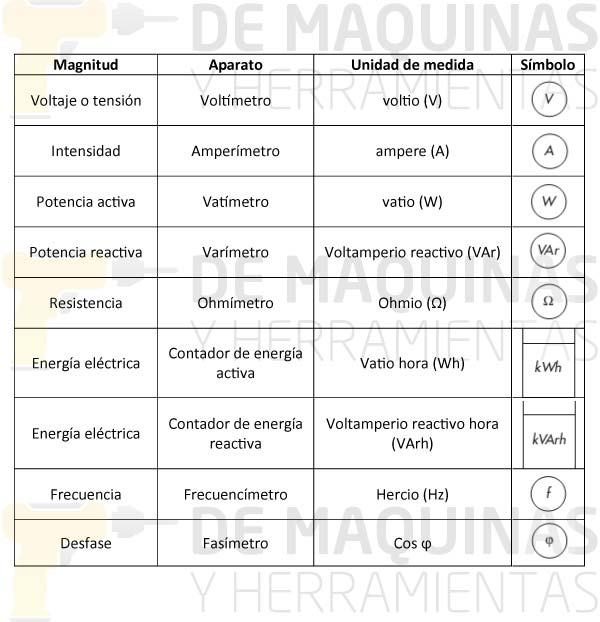
\includegraphics[width=0.55\textwidth]{img/magnitud-electrica.jpeg}
              \caption{Símbolos de magnitud eléctrica.}
              \label{fig:magnitud-electrica}
          \end{figure}

    \item \textbf{Clase de corriente:} Indica el tipo de corriente para el cual está diseñado el instrumento. En la Figura~\ref{fig:clase-corriente} se muestran los símbolos normalizados.
          \begin{figure}[H]
              \centering
              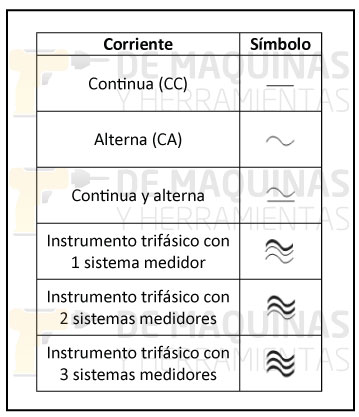
\includegraphics[width=0.35\textwidth]{img/clase-corriente.jpeg}
              \caption{Símbolos de clase de corriente.}
              \label{fig:clase-corriente}
          \end{figure}

    \item \textbf{Seguridad en la manipulación:} Las fallas de aislamiento pueden provocar una diferencia de potencial entre la caja del instrumento y sus partes metálicas con tierra. Por ello, los aparatos se someten a una tensión de prueba aplicada entre la caja y sus partes activas, que depende de la tensión nominal y se informa como \textit{tensión de prueba de aislamiento}. Se indica mediante una estrella con un número en su interior que representa dicha tensión en kilovoltios (kV). En la Figura~\ref{fig:tension-ensayo} se muestran algunos ejemplos.

          \begin{figure}[H]
              \centering
              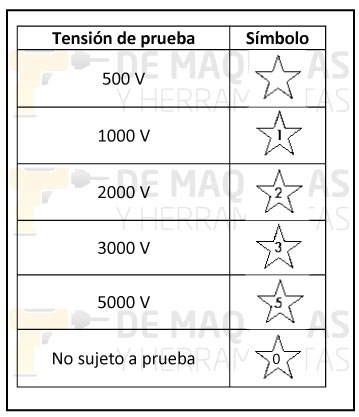
\includegraphics[width=0.4\textwidth]{img/tabla-tension-ensayo.jpeg}
              \caption{Ejemplos de símbolos de tensión de prueba de aislamiento.}
              \label{fig:tension-ensayo}
          \end{figure}

    \item \textbf{Posición de funcionamiento:} Indica la orientación en la que debe operar el instrumento para garantizar su precisión. En la Figura~\ref{fig:posicion-funcionamiento} se muestran los símbolos normalizados.
          \begin{figure}[H]
              \centering
              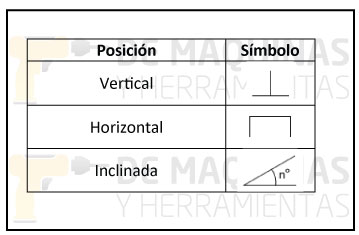
\includegraphics[width=0.35\textwidth]{img/posicion-funcionamiento.jpeg}
              \caption{Símbolos de posición de funcionamiento.}
              \label{fig:posicion-funcionamiento}
          \end{figure}

    \item \textbf{Clase de precisión:} Número que indica el error porcentual del instrumento (ver Figura~\ref{fig:clase-precision}). El cálculo del error asociado se desarrolla en la Sección~\ref{sec:errores}.
          \begin{figure}[H]
              \centering
              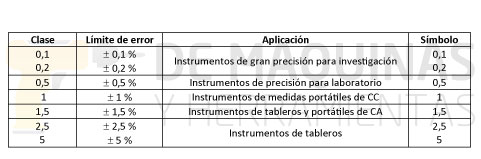
\includegraphics[width=0.5\textwidth]{img/clase-precision.jpeg}
              \caption{Símbolos de clase de precisión.}
              \label{fig:clase-precision}
          \end{figure}

    \item \textbf{Mecanismo de funcionamiento:} Mediante símbolos gráficos se distingue el principio de operación del instrumento. En la Figura~\ref{fig:mecanismo} se muestran los símbolos normalizados.
          \begin{figure}[H]
              \centering
              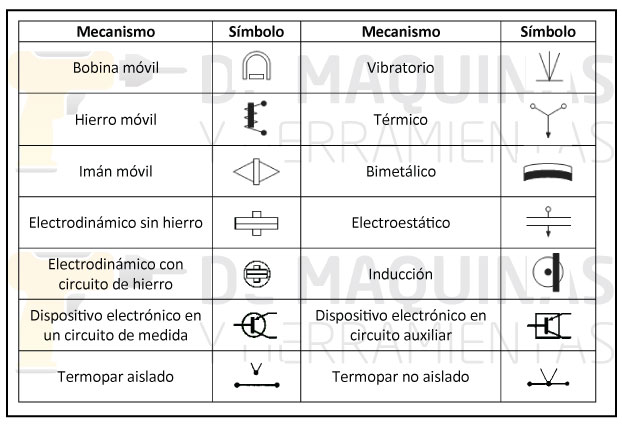
\includegraphics[width=0.5\textwidth]{img/mecanismo-funcionamiento.jpeg}
              \caption{Símbolos de mecanismo de funcionamiento.}
              \label{fig:mecanismo}
          \end{figure}
\end{enumerate}

\subsection{Errores de Medición}
\label{sec:errores}

Toda medición difiere del valor verdadero debido a imperfecciones en los instrumentos y métodos empleados. Los errores se clasifican en:

\begin{itemize}
    \item \textbf{Sistemáticos:} Son constantes y repetibles; pueden corregirse mediante calibración del instrumento.
    \item \textbf{Aleatorios:} Son variaciones impredecibles que se reducen mediante el promediado estadístico de múltiples mediciones.
\end{itemize}

Para cuantificar el error de un instrumento se utiliza el concepto de \textit{clase de precisión}. El error absoluto máximo está dado por:

\begin{equation}
    \varepsilon = \frac{\text{clase}}{100} \times A_{\text{máx}}
\end{equation}

donde $\text{clase}$ es la clase de precisión del instrumento y $A_{\text{máx}}$ es el alcance (valor máximo de la escala). El valor real $A_r$ se expresa entonces como:

\begin{equation}
    A_r = A_m \pm \varepsilon
\end{equation}

siendo $A_m$ el valor medido.

Según su precisión, los instrumentos se clasifican en:
\begin{itemize}
    \item \textbf{Instrumentos de precisión:} clases 0.1, 0.2, 0.5.
    \item \textbf{Instrumentos industriales:} clases 1, 1.5, 2.5, 5.
\end{itemize}

\subsection{Cifras Significativas}

La cantidad de cifras significativas con que debe reportarse un resultado está acotada por la precisión del instrumento. Reglas prácticas:

\begin{itemize}
    \item La primera cifra incierta del resultado coincide con la primera cifra del error.
    \item No deben reportarse más decimales de los que la resolución del instrumento permite.
    \item Ejemplo: si el error es $\pm 0.05$, el resultado debe expresarse con 2 decimales.
\end{itemize}
